%----------------------------------------------------------------------------------------
%	PACKAGES AND THEMES
%----------------------------------------------------------------------------------------
\pdfoutput=1
\documentclass{beamer}

\usepackage[utf8]{inputenc}
\usepackage[scaled]{helvet} %helvetica i sliden blir bra
\usepackage[T1]{fontenc}

\usepackage{graphicx} % Allows including images
\usepackage{booktabs} % Allows the use of \toprule, \midrule and \bottomrule in tables
\usepackage{comment}
\usepackage[swedish]{babel}
\usepackage{graphicx}
\usepackage{graphics}
\usepackage{units}
%\usepackage{siunitx} %SI-enheter
\usepackage{comment}
\usepackage{epstopdf}
\usepackage{tikz}
\usepackage{eso-pic}
\usepackage{wallpaper} %För bakgrundsbilder
\usepackage{multimedia}
\usepackage{media9}

\usepackage{physics}

\graphicspath{ 
{src_figures/Avancez/}  %specialbilder som bara behövs för bakgrunden
{presentation_figures/} %bilder som används i själva presentationen
}



\definecolor{CTHblue}{RGB}{00,00,102}   % Dessa är faktiskt officella Chalmersfärger som är beslutat att
\definecolor{CTHgrey}{RGB}{204,204,204} % de skall användas till presentationer. Andra är inte tillåtna...
\definecolor{CTHgreen}{RGB}{113,178,60} % citation needed []
\definecolor{CTHblack}{RGB}{00,00,00}


\mode<presentation> {

% The Beamer class comes with a number of default slide themes
% which change the colors and layouts of slides. Below this is a list
% of all the themes, uncomment each in turn to see what they look like.

%\usetheme{default}
%\usetheme{AnnArbor}
%\usetheme{Antibes}
%\usetheme{Bergen}
%\usetheme{Berkeley}
%\usetheme{Berlin}
%\usetheme{Boadilla}
%\usetheme{CambridgeUS}
%\usetheme{Copenhagen}
%\usetheme{Darmstadt}
%\usetheme{Dresden}
%\usetheme{Frankfurt}
%\usetheme{Goettingen}
%\usetheme{Hannover}
%\usetheme{Ilmenau}
%\usetheme{JuanLesPins}
%\usetheme{Luebeck}
%\usetheme{Madrid}
%\usetheme{Malmoe}
%\usetheme{Marburg}
%\usetheme{Montpellier}
%\usetheme{PaloAlto}
%\usetheme{Pittsburgh}
%\usetheme{Rochester}
%\usetheme{Singapore}
%\usetheme{Szeged}
%\usetheme{Warsaw}

% As well as themes, the Beamer class has a number of color themes
% for any slide theme. Uncomment each of these in turn to see how it
% changes the colors of your current slide theme.

%\usecolortheme{albatross}
%\usecolortheme{beaver}
%\usecolortheme{beetle}
%\usecolortheme{crane}
%\usecolortheme{dolphin}
%\usecolortheme{dove}
%\usecolortheme{fly}
%\usecolortheme{lily}
%\usecolortheme{orchid}
%\usecolortheme{rose}
%\usecolortheme{seagull}
%\usecolortheme{seahorse}
%\usecolortheme{whale}
%\usecolortheme{wolverine}

% \setbeamercolor*{palette primary}{fg=CTHgrey,bg=CTHblue}
% \setbeamercolor*{palette secondary}{fg=CTHblack,bg=CTHgrey}
% \setbeamercolor*{palette tertiary}{fg=CTHgrey,bg=CTHblack}

%\setbeamertemplate{footline} % To remove the footer line in all slides uncomment this line
%\setbeamertemplate{footline}[page number] % To replace the footer line in all slides with a simple slide count uncomment this line

%\setbeamertemplate{navigation symbols}{} % To remove the navigation symbols from the bottom of all slides uncomment this line
}



\newcommand{\RBox}[1]{%
  \tikz\node[draw,rounded corners,align=center,] {#1};%
}  

% \usebackgroundtemplate{\vbox to \paperheight{\vspace*{2pt}
\includegraphics[width=\paperwidth]{cth_fp.pdf}}}



\renewcommand{\thefootnote}{\fnsymbol{footnote}}

%----------------------------------------------------------------------------------------
%	TITLE PAGE
%----------------------------------------------------------------------------------------


\usetheme[titleflower=true]{chalmers} % titleflower = true or false
\title[Kort titel]{Lång titel som kommer på förstasidan} % Första klammern är en "short title"
\subtitle{} % optional
\author{Andréas Sundström } % [short author (optional)]{many authors}
\institute[Chalmers]{Chalmers tekniska högskla}
%\titlepageextra{IPT 2015, Warsaw} % Optional extra info, appears before date on title page
\footer{\insertshorttitle} % optional, manually sets footer (default is short author)
%\footer{Something completely different} % but it can of course be anything.

\titlepagelogofile{Avancez_black}
\date{\vspace{-0.25cm}}




\begin{document}

\begin{frame}[plain]

\linethickness{0.075mm}

  \titlepage
\end{frame}
% }







%%%%%%%%%%%%%%%%%%%%%%%%Här börjar presentationen%%%%%%%%%%%%%%%%%%%%%%%%


\begin{frame}
\frametitle{Innehåll}

\tableofcontents

\end{frame}




\section{Demoslides1 -- detta kommer med i innehållsförteckningen }
\begin{frame}
\frametitle{En titel till den här sliden}
 \begin{columns}[c]
\column{.4\textwidth} % Left column and width
Text här.
\begin{itemize}
    \item Ibland vill man ha punkter.
\end{itemize}
\column{.6\textwidth} % Right column and width
Den här sliden har två kolumner
\begin{figure}
%\includegraphics[width=1\textwidth]{}
% \caption{}
\end{figure}
\end{columns}
\end{frame}

\subsection{Man kan också ha lägre rubriknivåer}
\begin{frame}
\frametitle{Man kan ha flera frames i en section}
 \begin{columns}[c]
\column{.4\textwidth} % Left column and width
Mer text.
\begin{itemize}
    \item Fler punkter
\end{itemize}
\column{.6\textwidth} % Right column and width
Den här sliden har också två kolumner
\begin{figure}
%\includegraphics[width=1\textwidth]{}
% \caption{}
\end{figure}
\end{columns}
\end{frame}


\section{Demoslide2 -- detta kommer också med i sidfoten}
\begin{frame}
\frametitle{Ibland vill man kanske bara ha en kolumn}
Då hamnar texten över hela sidan istället. Särskit om man skriver på om massa onödigheter. Man ska helst undvika att ha med för mycket text på sin slide, för då hinner inte åskådaren läsa vad som står.

Men man kan behöva en hel slide om man ska lägga in någon stor och jobbig ekvation
\[
\sum_{k=0}^\infty \frac{\cos^2(\pi^k)+\sin^2(\pi^k)}{\int_0^\infty t^k\mathrm{e}^t \dd{t} } 
= \lim_{n\to\infty}\left(1+\frac{1}{n}\right)^n. 
\]

\end{frame}

\begin{frame}

\begin{figure}
\resizebox{.8\textwidth}{!}{% GNUPLOT: LaTeX picture with Postscript
\begingroup
  \makeatletter
  \providecommand\color[2][]{%
    \GenericError{(gnuplot) \space\space\space\@spaces}{%
      Package color not loaded in conjunction with
      terminal option `colourtext'%
    }{See the gnuplot documentation for explanation.%
    }{Either use 'blacktext' in gnuplot or load the package
      color.sty in LaTeX.}%
    \renewcommand\color[2][]{}%
  }%
  \providecommand\includegraphics[2][]{%
    \GenericError{(gnuplot) \space\space\space\@spaces}{%
      Package graphicx or graphics not loaded%
    }{See the gnuplot documentation for explanation.%
    }{The gnuplot epslatex terminal needs graphicx.sty or graphics.sty.}%
    \renewcommand\includegraphics[2][]{}%
  }%
  \providecommand\rotatebox[2]{#2}%
  \@ifundefined{ifGPcolor}{%
    \newif\ifGPcolor
    \GPcolortrue
  }{}%
  \@ifundefined{ifGPblacktext}{%
    \newif\ifGPblacktext
    \GPblacktexttrue
  }{}%
  % define a \g@addto@macro without @ in the name:
  \let\gplgaddtomacro\g@addto@macro
  % define empty templates for all commands taking text:
  \gdef\gplbacktext{}%
  \gdef\gplfronttext{}%
  \makeatother
  \ifGPblacktext
    % no textcolor at all
    \def\colorrgb#1{}%
    \def\colorgray#1{}%
  \else
    % gray or color?
    \ifGPcolor
      \def\colorrgb#1{\color[rgb]{#1}}%
      \def\colorgray#1{\color[gray]{#1}}%
      \expandafter\def\csname LTw\endcsname{\color{white}}%
      \expandafter\def\csname LTb\endcsname{\color{black}}%
      \expandafter\def\csname LTa\endcsname{\color{black}}%
      \expandafter\def\csname LT0\endcsname{\color[rgb]{1,0,0}}%
      \expandafter\def\csname LT1\endcsname{\color[rgb]{0,1,0}}%
      \expandafter\def\csname LT2\endcsname{\color[rgb]{0,0,1}}%
      \expandafter\def\csname LT3\endcsname{\color[rgb]{1,0,1}}%
      \expandafter\def\csname LT4\endcsname{\color[rgb]{0,1,1}}%
      \expandafter\def\csname LT5\endcsname{\color[rgb]{1,1,0}}%
      \expandafter\def\csname LT6\endcsname{\color[rgb]{0,0,0}}%
      \expandafter\def\csname LT7\endcsname{\color[rgb]{1,0.3,0}}%
      \expandafter\def\csname LT8\endcsname{\color[rgb]{0.5,0.5,0.5}}%
    \else
      % gray
      \def\colorrgb#1{\color{black}}%
      \def\colorgray#1{\color[gray]{#1}}%
      \expandafter\def\csname LTw\endcsname{\color{white}}%
      \expandafter\def\csname LTb\endcsname{\color{black}}%
      \expandafter\def\csname LTa\endcsname{\color{black}}%
      \expandafter\def\csname LT0\endcsname{\color{black}}%
      \expandafter\def\csname LT1\endcsname{\color{black}}%
      \expandafter\def\csname LT2\endcsname{\color{black}}%
      \expandafter\def\csname LT3\endcsname{\color{black}}%
      \expandafter\def\csname LT4\endcsname{\color{black}}%
      \expandafter\def\csname LT5\endcsname{\color{black}}%
      \expandafter\def\csname LT6\endcsname{\color{black}}%
      \expandafter\def\csname LT7\endcsname{\color{black}}%
      \expandafter\def\csname LT8\endcsname{\color{black}}%
    \fi
  \fi
  \setlength{\unitlength}{0.0500bp}%
  \begin{picture}(7200.00,5040.00)%
    \gplgaddtomacro\gplfronttext{%
      \csname LT0\endcsname%
      \put(264,4930){\makebox(0,0)[l]{\strut{}epslatex  terminal test}}%
      \csname LT3\endcsname%
      \put(2280,2520){\makebox(0,0)[l]{\strut{}12345678901234567890}}%
      \put(2280,2828){\makebox(0,0)[l]{\strut{}test of character width:}}%
      \csname LTb\endcsname%
      \put(3600,3840){\makebox(0,0)[l]{\strut{}left justified}}%
      \put(3600,3620){\makebox(0,0){\strut{}centre+d text}}%
      \put(3600,3400){\makebox(0,0)[r]{\strut{}right justified}}%
      \csname LT1\endcsname%
      \put(220,2520){\rotatebox{-270}{\makebox(0,0){\strut{}rotated ce+ntred text}}}%
      \put(660,2520){\rotatebox{45}{\makebox(0,0)[l]{\strut{} rotated by +45 deg}}}%
      \put(440,2520){\rotatebox{-45}{\makebox(0,0)[l]{\strut{} rotated by -45 deg}}}%
      \csname LT4\endcsname%
      \put(3468,4804){\makebox(0,0)[r]{\strut{}show ticscale}}%
      \csname LTb\endcsname%
      \put(6345,4820){\makebox(0,0)[r]{\strut{}-1}}%
      \csname LTa\endcsname%
      \put(6345,4600){\makebox(0,0)[r]{\strut{}0}}%
      \csname LT0\endcsname%
      \put(6345,4380){\makebox(0,0)[r]{\strut{}1}}%
      \csname LT1\endcsname%
      \put(6345,4160){\makebox(0,0)[r]{\strut{}2}}%
      \csname LT2\endcsname%
      \put(6345,3940){\makebox(0,0)[r]{\strut{}3}}%
      \csname LT3\endcsname%
      \put(6345,3720){\makebox(0,0)[r]{\strut{}4}}%
      \csname LT4\endcsname%
      \put(6345,3500){\makebox(0,0)[r]{\strut{}5}}%
      \csname LT5\endcsname%
      \put(6345,3280){\makebox(0,0)[r]{\strut{}6}}%
      \csname LT6\endcsname%
      \put(6345,3060){\makebox(0,0)[r]{\strut{}7}}%
      \csname LT7\endcsname%
      \put(6345,2840){\makebox(0,0)[r]{\strut{}8}}%
      \csname LT8\endcsname%
      \put(6345,2620){\makebox(0,0)[r]{\strut{}9}}%
      \csname LT0\endcsname%
      \put(6345,2400){\makebox(0,0)[r]{\strut{}10}}%
      \csname LT1\endcsname%
      \put(6345,2180){\makebox(0,0)[r]{\strut{}11}}%
      \csname LT2\endcsname%
      \put(6345,1960){\makebox(0,0)[r]{\strut{}12}}%
      \csname LT3\endcsname%
      \put(6345,1740){\makebox(0,0)[r]{\strut{}13}}%
      \csname LT4\endcsname%
      \put(6345,1520){\makebox(0,0)[r]{\strut{}14}}%
      \csname LT5\endcsname%
      \put(6345,1300){\makebox(0,0)[r]{\strut{}15}}%
      \csname LT6\endcsname%
      \put(6345,1080){\makebox(0,0)[r]{\strut{}16}}%
      \csname LT7\endcsname%
      \put(6345,860){\makebox(0,0)[r]{\strut{}17}}%
      \csname LT8\endcsname%
      \put(6345,640){\makebox(0,0)[r]{\strut{}18}}%
      \csname LT0\endcsname%
      \put(6345,420){\makebox(0,0)[r]{\strut{}19}}%
      \csname LTb\endcsname%
      \put(1260,201){\makebox(0,0)[l]{\strut{}  lw 1}}%
      \put(1260,402){\makebox(0,0)[l]{\strut{}  lw 2}}%
      \put(1260,603){\makebox(0,0)[l]{\strut{}  lw 3}}%
      \put(1260,804){\makebox(0,0)[l]{\strut{}  lw 4}}%
      \put(1260,1005){\makebox(0,0)[l]{\strut{}  lw 5}}%
      \put(1260,1206){\makebox(0,0)[l]{\strut{}  lw 6}}%
      \put(540,1407){\makebox(0,0)[l]{\strut{}linewidth}}%
      \put(4860,960){\makebox(0,0){\strut{}pattern fill}}%
      \put(3690,740){\makebox(0,0){\strut{} 0}}%
      \put(3960,740){\makebox(0,0){\strut{} 1}}%
      \put(4230,740){\makebox(0,0){\strut{} 2}}%
      \put(4500,740){\makebox(0,0){\strut{} 3}}%
      \put(4770,740){\makebox(0,0){\strut{} 4}}%
      \put(5040,740){\makebox(0,0){\strut{} 5}}%
      \put(5310,740){\makebox(0,0){\strut{} 6}}%
      \put(5580,740){\makebox(0,0){\strut{} 7}}%
      \put(5850,740){\makebox(0,0){\strut{} 8}}%
      \put(6120,740){\makebox(0,0){\strut{} 9}}%
      \csname LTb\endcsname%
      \put(5040,4653){\makebox(0,0){\strut{}filled polygons:}}%
    }%
    \gplbacktext
    \put(0,0){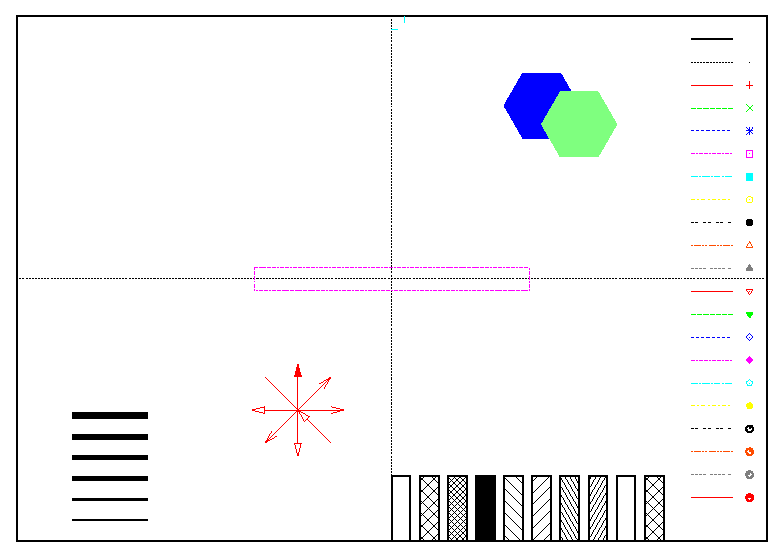
\includegraphics{fig0}}%
    \gplfronttext
  \end{picture}%
\endgroup
}
% \caption{}
\end{figure}

\end{frame}

\end{document}
